

\subsection{Term Structure of Interest Rates}
According to definition on INVESTOPEDIA, "the term structure of interest rates is the relationship between interest rates or bond yields and different terms or maturities. The term structure of interest rates is also known as a yield curve and it plays central role in an economy. The term structure reflects expectations of market participants about future changes in interest rates and their assessment of monetory policy conditions"\\
In mathematical finance, the term structure of interest rates is often modeled using stochastic methods, which can pose a number of difficult problems for estimation. One of the most crucial problems is that the parameters enter the state space in a highly nonlinear fasion. However, solving these non-linear systems are often quite rewarding as we can derive bonds and their derivatives prices from the models, yet, most of the time, we can only use MCMC methods to help solving the system.
\subsection{Vasicek's Model With Jumps}
The Vasicek's model assumes that the instantaneous spot rate is a Gaussian diffusion:
\begin{align*}
  dr_t &= \kappa_r(\theta_r-r_t)dt+\sigma_rdW_t^r\\
  dr_t &= (a_r+b_r r_t)dt+\sigma_rdW_t^r
\end{align*}
where $W_t^r$ is a Brownian motion under the objective measure, $P$, and we will work with the $(a_r,b_r)$ parameterization of the drift. \\
Baz and Das (1996) consider an extension of Vasicek's model to incorporate jumps in the short rate:
$$dr_t=(a_r-b_rr_{t-})dt +\sigma_r dW_t^r + d\left(\sum\limits_{j=1}^{N_t}\xi_{\tau_j}\right)$$
where we assume that $N_t$ is a Poisson process with constant intensity $\lambda$ and the jumps sizes are i.i.d. normal $\xi_{\tau_j}\sim N(\mu_J,\sigma_J^2)$. To value bonds under this model, we assume that the market price of interest rate risk is $\lambda_t=\lambda_r\sqrt{r_t}$  and if we assume the diffusive risk premium is constant, that $N_t^Q$ is a Poisson process under $Q$ with constant intensity $\lambda^Q$ and that the jump sizes are normally distributed under $Q$, $\xi_{\tau_j}^Q\sim N\left(\mu_j^Q,(\sigma_J^2)^Q\right)$, the evolution of the spot rate under $Q$ is then
$$dr_t = \kappa_r(\theta_r^Q-r_t)dt+\sigma_rdW_t^r(Q)+d\left(\sum\limits_{j=1}^{N_t^Q}\xi_{\tau_j}^Q\right)$$
where $W_t^r(Q)$ is a standard Brownian motion under the equivalent martingale measure $Q$. Then under this model, Using Feyman Kac's theorem, the price a non-defaultable zero coupon bond is given by
$$P(r_t,\tau)=E_t^Q\left[e^{-\int_t^{t+\tau}r_sds}\right]$$
\subsection{Monte Carlo Simulation and Integration Implementation}
In this mini-project, we assume the following parameter values 
\begin{align*}
  \tau &= 10\\
  \theta_r^Q &= 0.04\\
  r_t &= 0.015\\
  \kappa_r &= 0.6\\
  \sigma_r &= 0.03\\
  \lambda^Q &= 2\\
  \mu_J^Q &= 0\\
  (\sigma_J^2)^Q &= 0.01
\end{align*}
For small $h$, at any instance $t$, the distribution of $r_{t+h}$ given $r_t$ follows 
$$f(r_{t+h}|r_t) \sim N(r_t+\kappa_r(\theta_r^Q-r_t)h,(\sigma_r^2)^Q\sqrt{h}+Bernuolli(\lambda^Qh)*N\left(\mu_J^Q,(\sigma_J^2)^Q\right)$$
Using the distribution above, we simulate $M=2000$ paths and use Monte Carlo integration techiniques to calculate the price of zero-coupon bond. Ten runs are executed to investigate the consistency of the estimate.\\
Source code:\\
\begin{knitrout}
\definecolor{shadecolor}{rgb}{0.969, 0.969, 0.969}\color{fgcolor}\begin{kframe}
\begin{alltt}
\hlcom{#calculate the price of zero coupon bonds with Vasicek}
\hlcom{#with jump models}

\hlcom{#financial parameters (all adjusted for risk neutral measure)}
\hlstd{T} \hlkwb{=} \hlnum{10}
\hlstd{theta} \hlkwb{=} \hlnum{0.04}
\hlstd{cr} \hlkwb{=} \hlnum{0.015}
\hlstd{kappa} \hlkwb{=} \hlnum{0.6}
\hlstd{sigma} \hlkwb{=} \hlnum{0.03}
\hlstd{lambda} \hlkwb{=} \hlnum{2}
\hlstd{sigmaj} \hlkwb{=} \hlnum{0.01}
\hlstd{muj} \hlkwb{=} \hlnum{0}

\hlcom{#time interval set to be 0.01 to make 100 intervals per year}
\hlstd{h}\hlkwb{=}\hlnum{0.01}
\hlstd{M} \hlkwb{=} \hlnum{2000}
\hlstd{num} \hlkwb{=} \hlkwd{round}\hlstd{(T}\hlopt{/}\hlstd{h)}
\hlstd{vallist} \hlkwb{=} \hlkwd{rep}\hlstd{(}\hlnum{0}\hlstd{,M)}
\hlstd{plotX} \hlkwb{=} \hlkwd{matrix}\hlstd{(}\hlkwc{nrow} \hlstd{=} \hlnum{20}\hlstd{,} \hlkwc{ncol} \hlstd{= num}\hlopt{+}\hlnum{1}\hlstd{)}
\hlkwa{for} \hlstd{(j} \hlkwa{in} \hlnum{1}\hlopt{:}\hlstd{M) \{}
  \hlstd{X} \hlkwb{=} \hlkwd{rep}\hlstd{(}\hlnum{0}\hlstd{,num}\hlopt{+}\hlnum{1}\hlstd{)}
  \hlstd{X[}\hlnum{1}\hlstd{]} \hlkwb{=} \hlstd{cr}
  \hlkwa{for} \hlstd{(i} \hlkwa{in} \hlnum{1}\hlopt{:}\hlstd{num) \{}
    \hlkwa{if} \hlstd{(}\hlkwd{runif}\hlstd{(}\hlnum{1}\hlstd{)}\hlopt{<}\hlstd{lambda}\hlopt{*}\hlstd{h) \{jump} \hlkwb{=} \hlkwd{rnorm}\hlstd{(}\hlnum{1}\hlstd{,muj,sigmaj)\}}
    \hlkwa{else} \hlstd{jump} \hlkwb{=} \hlnum{0}
    \hlstd{X[i}\hlopt{+}\hlnum{1}\hlstd{]} \hlkwb{=} \hlkwd{rnorm}\hlstd{(}\hlnum{1}\hlstd{,X[i]}\hlopt{+}\hlstd{kappa}\hlopt{*}\hlstd{(theta}\hlopt{-}\hlstd{X[i])}\hlopt{*}\hlstd{h,sigma}\hlopt{*}\hlkwd{sqrt}\hlstd{(h))}\hlopt{+}\hlstd{jump}
    \hlkwa{if} \hlstd{(j}\hlopt{<=}\hlnum{20}\hlstd{) plotX[j,]} \hlkwb{=} \hlstd{X}
  \hlstd{\}}
  \hlstd{vallist[j]} \hlkwb{=} \hlkwd{exp}\hlstd{(}\hlopt{-}\hlkwd{sum}\hlstd{(X)}\hlopt{*}\hlstd{h)}
\hlstd{\}}
\hlstd{price} \hlkwb{=} \hlkwd{mean}\hlstd{(vallist)}
\hlstd{se} \hlkwb{=} \hlkwd{sd}\hlstd{(vallist)}\hlopt{/}\hlkwd{sqrt}\hlstd{(M)}
\hlkwd{cat}\hlstd{(}\hlstr{'The estimated zero-coupon bond price is '}\hlstd{,price,}\hlstr{'\textbackslash{}n'}\hlstd{)}
\hlkwd{cat}\hlstd{(}\hlstr{'The standard error is '}\hlstd{,se,}\hlstr{'\textbackslash{}n'}\hlstd{)}
\end{alltt}
\end{kframe}
\end{knitrout}
Output of several runs:
\begin{knitrout}
\definecolor{shadecolor}{rgb}{0.969, 0.969, 0.969}\color{fgcolor}\begin{kframe}
\begin{verbatim}
## The estimated zero-coupon bond price is  0.7043499 
## The standard error is  0.002424588
## The estimated zero-coupon bond price is  0.706554 
## The standard error is  0.002378813
## The estimated zero-coupon bond price is  0.7110355 
## The standard error is  0.002479945
## The estimated zero-coupon bond price is  0.7031318 
## The standard error is  0.002333143
## The estimated zero-coupon bond price is  0.7018515 
## The standard error is  0.002379074
## The estimated zero-coupon bond price is  0.7057709 
## The standard error is  0.002414406
## The estimated zero-coupon bond price is  0.7024047 
## The standard error is  0.002393151
## The estimated zero-coupon bond price is  0.7087772 
## The standard error is  0.002428283
## The estimated zero-coupon bond price is  0.7051398 
## The standard error is  0.002356732
## The estimated zero-coupon bond price is  0.7117877 
## The standard error is  0.00238904
\end{verbatim}
\end{kframe}
\end{knitrout}
The tabulated result is as follows:\\
\begin{center}
\begin{knitrout}
\definecolor{shadecolor}{rgb}{0.969, 0.969, 0.969}\color{fgcolor}
\begin{tabular}{r|r}
\hline
estprice & estse\\
\hline
0.7043499 & 0.0024246\\
\hline
0.7065540 & 0.0023788\\
\hline
0.7110355 & 0.0024799\\
\hline
0.7031318 & 0.0023331\\
\hline
0.7018515 & 0.0023791\\
\hline
0.7057709 & 0.0024144\\
\hline
0.7024047 & 0.0023932\\
\hline
0.7087772 & 0.0024283\\
\hline
0.7051398 & 0.0023567\\
\hline
0.7117877 & 0.0023890\\
\hline
\end{tabular}


\end{knitrout}
\end{center}
From the table above, we can see that the estimated price is fairly consistent with a mean of 0.7060803. The standard error of the price is also relatively small, the mean of the estimated standard error is 0.0023977. The standard error calculated from multiple runs of executing the program is 0.0034751. The small standar error of the estimated price means our MC estimation is reasonably accurate. \\
There are several advantages to this approach.\\
First of all, since there are multiple sources of stochasticity in our model (namely, the diffusive brownian motion, the number of jumps and the size jumps), solving the system analytically is (almost) impossible. In order to find a reasonable bond price under this model, we have to use MC simulation method.\\
Also, since we have simulated paths of realizations of the spot rate, we can also find out how risky the bond is. That is, if we invest the same amount in the bank account and follow the simulated spot rate paths, how much more or less we are going to make in comparison to investing in the zero-coupon bond. \\
Last but not least, we can look at some sample paths of the spot rate curve to see if our model assumption is valid. The following figure outlines 20 sample paths from our simulation
\begin{figure}[H]
  \centering
\begin{knitrout}
\definecolor{shadecolor}{rgb}{0.969, 0.969, 0.969}\color{fgcolor}
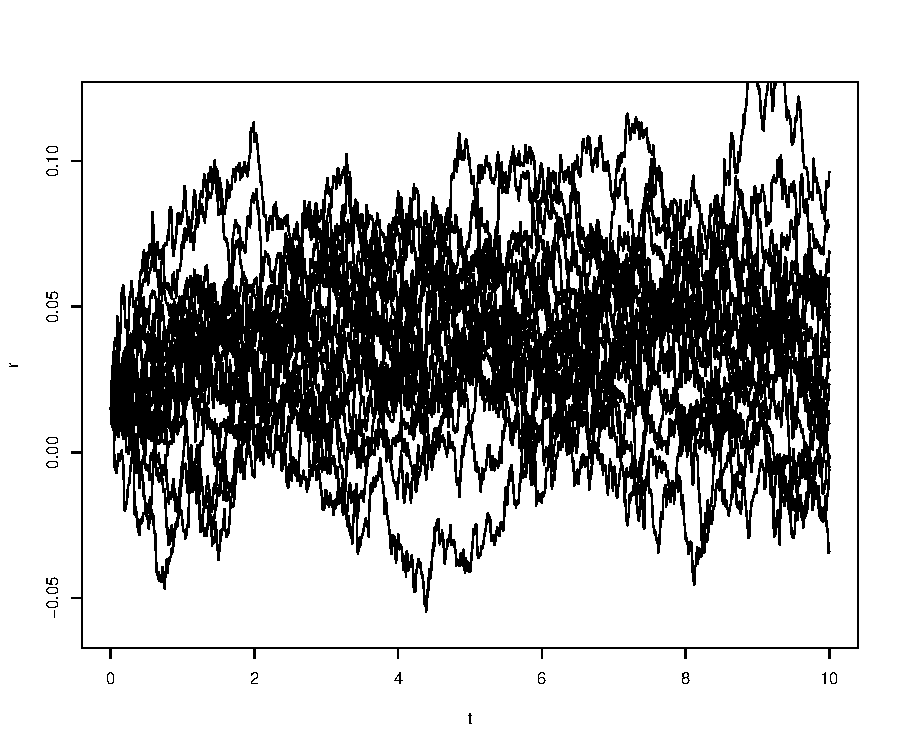
\includegraphics[width=\maxwidth]{figure/p10plot-1} 

\end{knitrout}
		\caption{20 simulated paths of the spot rate under risk neutral measure}
\end{figure}
From the figure above, we observe that the simulated paths follow typical strucure of actual observed spot rate curves. This validates to some extent that our model assumption is valid. 
\subsection{Further Research}
The original plan was actually to work on more advanced Monte Carlo method to estimate zero-coupon bond prices under this model assumption. However, the paper I was reading on this subject was quite intense, and I did not fully understand the methods described in the paper (and marking midterm papers for other courses is taking way longer than I have expected). In the paper, the financial parameters are not assumed to be known in advance, and the only given data in the implementation is the actual observed bond prices with different maturity. The spot rates and the parameters are assumed to follow a complicated joint distribution, so metroplis (or other sampling algorithms) have to be used to obtain the term structure curves. Here is the link to the referenced paper (\url{https://www0.gsb.columbia.edu/mygsb/faculty/research/pubfiles/564/MCMC.pdf})
